\documentclass[11pt, a4paper]{article}


\usepackage[english,francais]{babel}
\usepackage[utf8]{inputenc}
\usepackage[T1]{fontenc}
\usepackage[pdftex]{graphicx}
\usepackage{setspace}
\usepackage{hyperref}
\usepackage[french]{varioref}
\usepackage{amsfonts}
\usepackage{amssymb}
\usepackage[french,ruled]{algorithm2e}
\usepackage{amsmath}    % align

\usepackage{geometry}
\geometry{hscale=0.75,vscale=0.75,centering}

\title{TP1 - Sous-séquences maximales}
\author{Sébastien Delecraz \and \'Eloi Perdereau}
%\date{}


\begin{document}

\maketitle

\begin{abstract}
  Ce rapport propose une étude de différents algorithmes pour résoudre le
  problème du calcul de la sous-séquence de somme maximale dans un tableau
  d'entier. Quatre algorithmes de complexité différentes sont présentés ici.
  On trouvera donc pour chacun leur pseudo-code et une étude de leur
  complexité. Enfin nous confronterons les
  différents résultats obtenus et l'analyse théorique réalisée.
\end{abstract}

\section{Algorithme naïf}
\subsection{Pseudo-code}

\begin{algorithm}[H]
  \Entree{T, n}
  \Sortie{Sous-séquence maximale}
  \Deb{
    $S_{max} \leftarrow -\infty$ \\
    \PourTous{$1 \leq k \leq n$}{
      \PourTous{$k \leq l \leq n$}{
        $S \leftarrow 0$ \\
        \PourTous{$k \leq j \leq l$}{
          $S \leftarrow S + T[j]$
        }
        \Si{$S > S_{max}$}{$S_{max} \leftarrow S$}
      }
    }
    \Retour{$S_{max}$}
  }
  \caption{Naïf}
\end{algorithm}
\subsection{Complexité}
L'algorithme se compose de trois boucles de parcours du tableau imbriquées. Sa
complexité dans le pire des cas est donc :
\[C(n) = \Theta{(n^3)}\]

\section{Algorithme moins naïf}
\subsection{Pseudo-code}

\begin{algorithm}[H]
  \Entree{T, n}
  \Sortie{Sous-séquence maximale}
  \Deb{
    $S_{max} \leftarrow -\infty$ \\
    \PourTous{$1 \leq k \leq n$}{
      $S \leftarrow 0$ \\
      \PourTous{$k \leq l \leq n$}{
        $S \leftarrow S + T[l]$ \\
        \Si{$S > S_{max}$}{$S_{max} \leftarrow S$}
      }
    }
    \Retour{$S_{max}$}
  }
  \caption{Moins naïf}
\end{algorithm}
\subsection{Complexité}
L'algorithme se compose de deux boucles de parcours du tableau imbriquées. Sa
complexité dans le pire des cas est donc :
\[C(n) = \Theta{(n^2)}\]

\section{Algorithme diviser pour régner}
\subsection{Pseudo-code}

\begin{algorithm}[H]
  \Entree{T, k, l}
  \Sortie{Sous-séquence maximale}
  \Deb{
    \lSi{$l-k = 1$}{\Retour{$T[k]$}}
    \lSi{$l-k = 2$}{\Retour{max\{$T[k]$, $T[k+1]$, $T[k]+T[k+1]$\}}}
    $j \leftarrow \frac{l - k}{2}$ \\
    $S_1 \leftarrow Diviser\_pour\_regner (T, k, j)$ \\
    $S_2 \leftarrow Diviser\_pour\_regner (T, j+1, l)$ \\
    $S_3 \leftarrow S_{tmp} \leftarrow T[j]$ \\
    \Pour{i variant de j-1 à k descendant}{
      $S_{tmp} \leftarrow S_{tmp} + T[i]$ \\
      \Si{$S_{tmp} > S_3$}{$S_3 \leftarrow S_{tmp}$}
    }
    $S_4 \leftarrow S_{tmp} \leftarrow T[j]$ \\
    \Pour{i variant de j+1 à l-1 montant}{
      $S_{tmp} \leftarrow S_{tmp} + T[i]$ \\
      \Si{$S_{tmp} > S_4$}{$S_4 \leftarrow S_{tmp}$}
    }
    $S_0 \leftarrow S_3 + S_4 - T[j]$ \\
    \Retour{$max\{S_0, S_1, S_2\}$}
  }
  \caption{Diviser pour régner}
\end{algorithm}
\subsection{Complexité}
Cet algorithme applique la méthode diviser pour régner. On peut écrire son
équation de récurrence :
\begin{align*}
  C(n) & = 2*C(n/2) + 2*(n/2) \\
       & = 2*C(n/2) + \Theta{(n)}
\end{align*}
On applique ensuite le Master Theorem : \\
$c = \log_2 2 = 1$ \\
$f(n) = \Theta{(n)}$ \\
On est dans le cas 2 car $f(n) = \Theta{(n^c)}$. Donc la complexité de
l'algorithme est :
\[ C(n) = \Theta{(n \log n)} \]

\section{Algorithme incrémental}
\subsection{Pseudo-code}

\begin{algorithm}[H]
  \Entree{T, n}
  \Sortie{Sous-séquence maximale}
  \Deb{
    $S_{max} \leftarrow T[1]$ \\
    $S_1 \leftarrow 0$ \\
    $S_2 \leftarrow 0$ \\
    $maj \leftarrow false$ \\
    \PourTous{$2 \leq i \leq n$}{
      $S_1 \leftarrow S_1 + T[i]$ \\
      $S_2 \leftarrow S_2 + T[i]$ \\
      \Si{$T[i] < 0$}{
        \Si{$T[i] > S_{max}$}{
          $S_{max} \leftarrow T[i]$ \\
          $S_1 \leftarrow 0$ \\
          $S_2 \leftarrow 0$ \\
        }
        \Si{$S_2 < 0$}{
          $S_2 \leftarrow 0$ \\
        }
      }
      \Sinon{
        $S_{tmp} \leftarrow S_{max}$\\
        \Si{$S_1 + S_{tmp} > S_{tmp}$}{
          $S_{max} \leftarrow S_{max} + S_1$ \\
          $maj \leftarrow true$ \\
        }
        \Si{$S_2 > S_{tmp} \&\& S_2 > S_1 + S_{tmp}$}{
          $S_{max} \leftarrow S_2$ \\
          $maj \leftarrow true$ \\
        }
        \Si{$maj == true$}{
          $S_1 \leftarrow 0$ \\
          $S_2 \leftarrow 0$ \\
        }
      }
    }
    % \Retour{$S_{max}$}
  }
  \caption{Incrémental}
\end{algorithm}
\subsection{Complexité}
L'algorithme ne parcours qu'une seule fois le tableau d'entrée. Sa
complexité dans le pire des cas est donc :
\[C(n) = n = \Theta{(n)}\]

\newpage
\section{Résulats expérimentaux}

Les performances de chaque algorithme sont données individuellement en
annexes. \\

Le graphique ci dessous nous montre pour chaque algorithme leur temps
d'execution en fonction de la taille des instances données en entrée.

\begin{figure}[h]
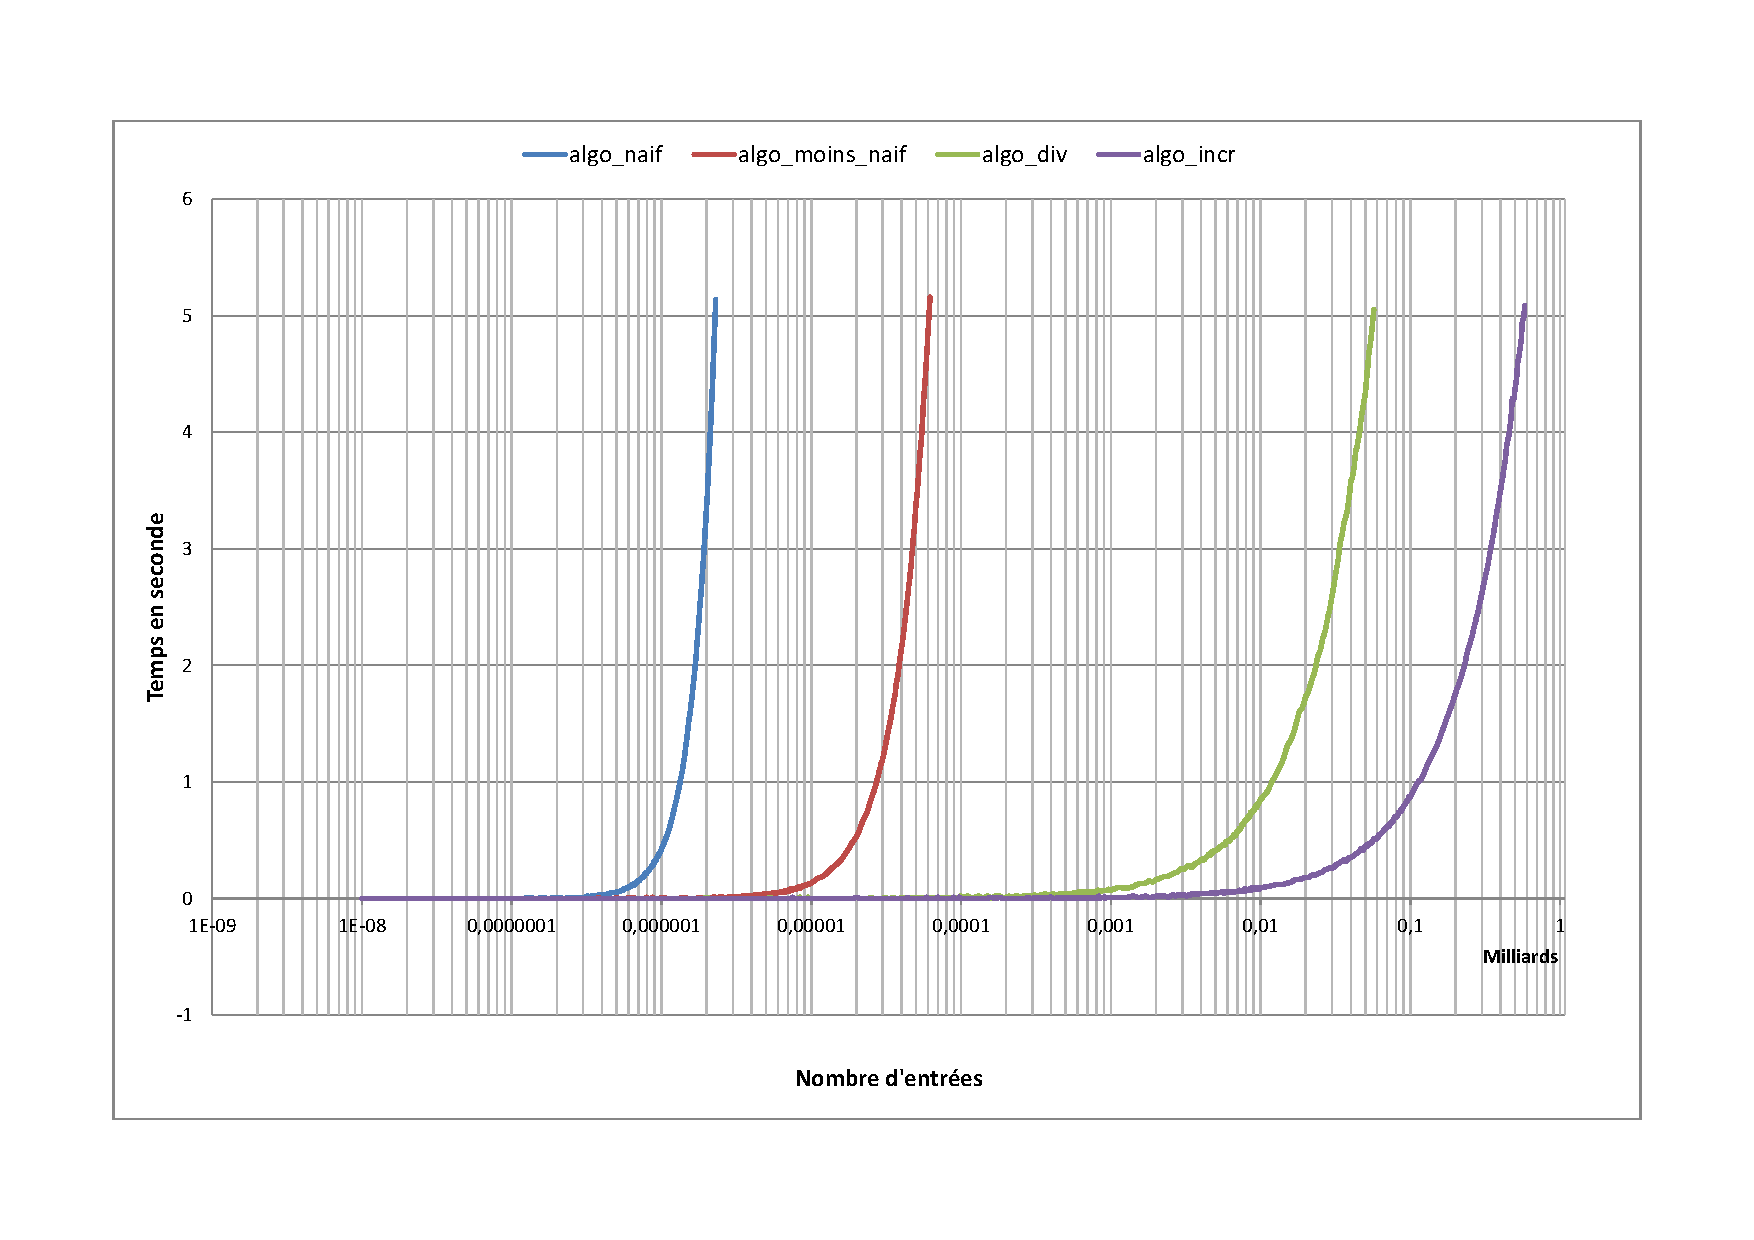
\includegraphics [scale=0.5]{images/comparatif.png}
\caption{Évolution des perfomances des algorithmes}
\end{figure}

On constate une différence de performances qui correspond bien à l'analyse de
complexité effectuée.
\[ \Theta{(n^3)} > \Theta{(n^2)} > \Theta{(n \log n)} > \Theta{(n)} \]

\appendix

\begin{figure}[h]
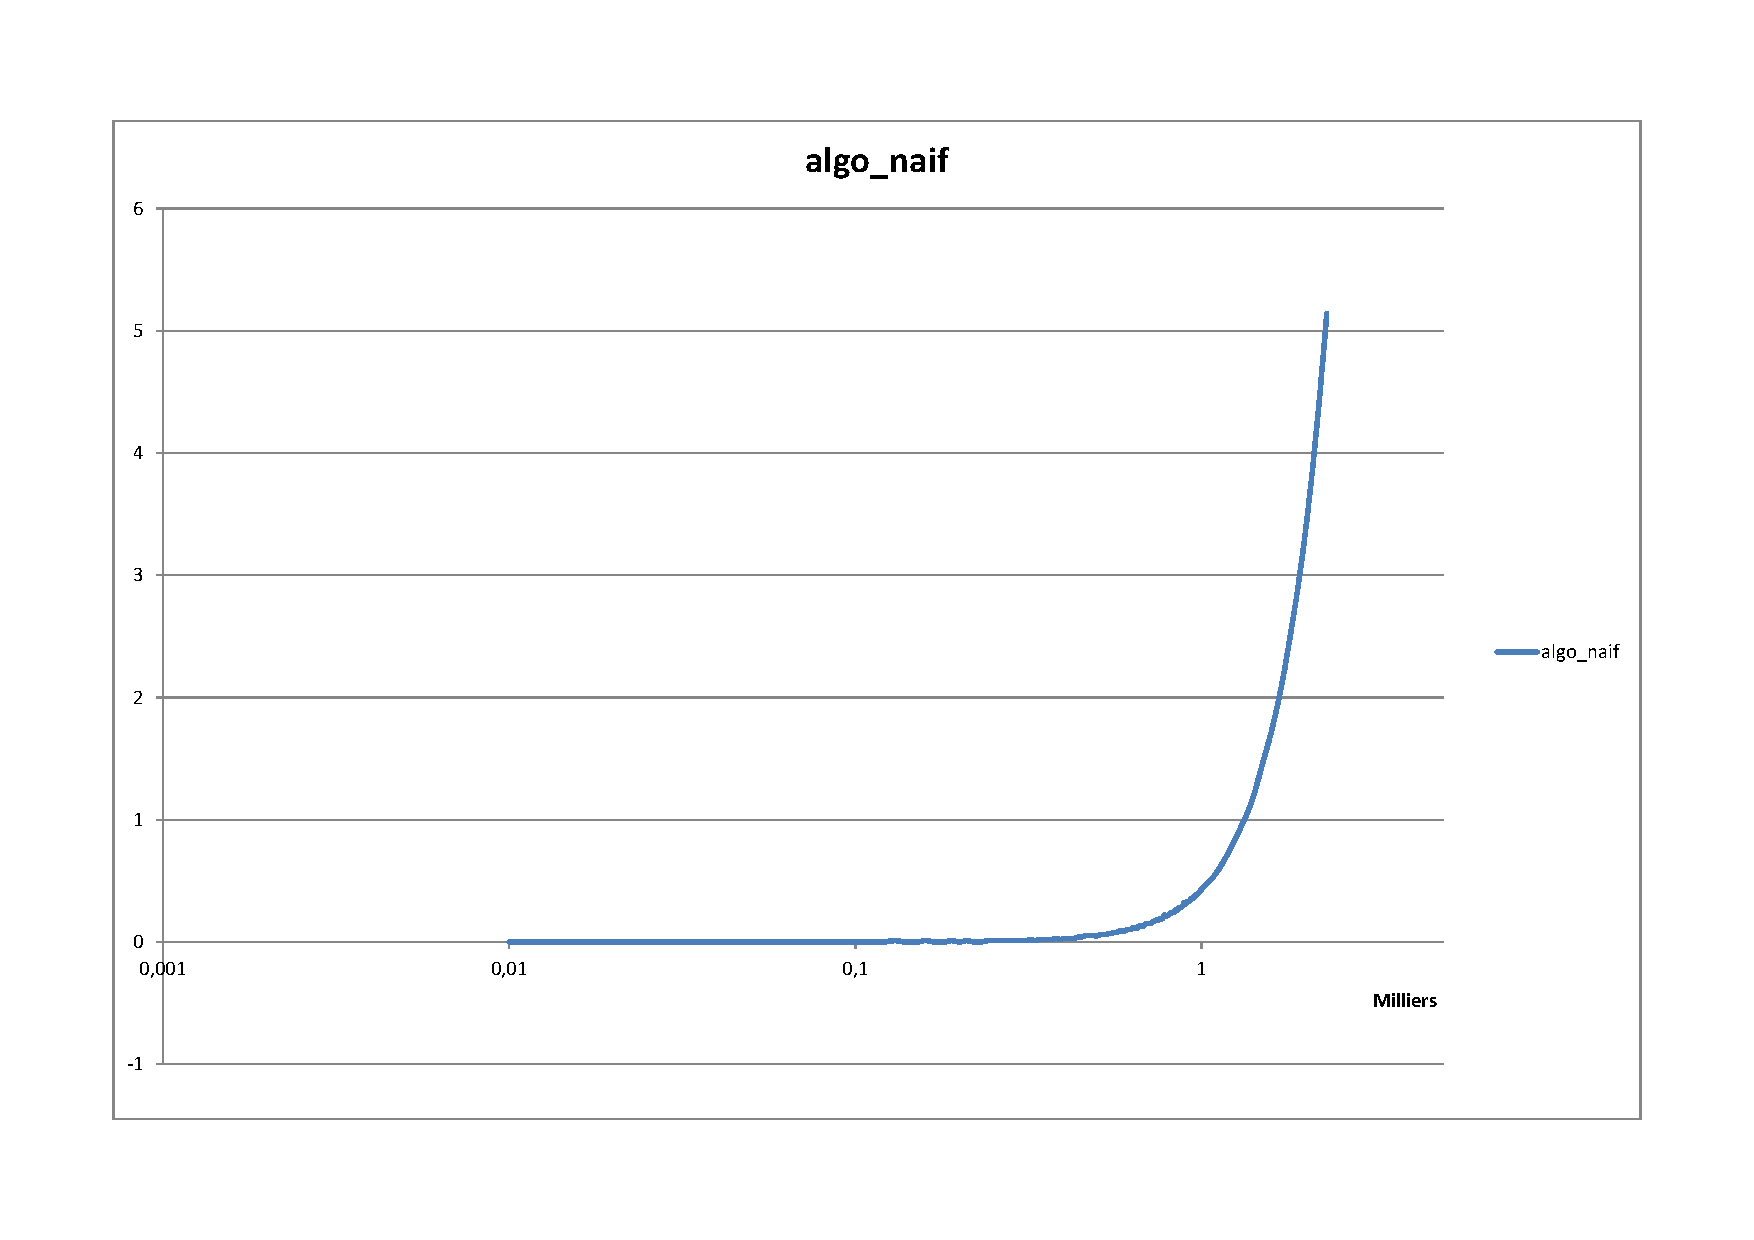
\includegraphics [scale=0.5]{images/algo_naif.png}
\caption{Performances de l'algorithme naïf}
\end{figure}

\begin{figure}[h]
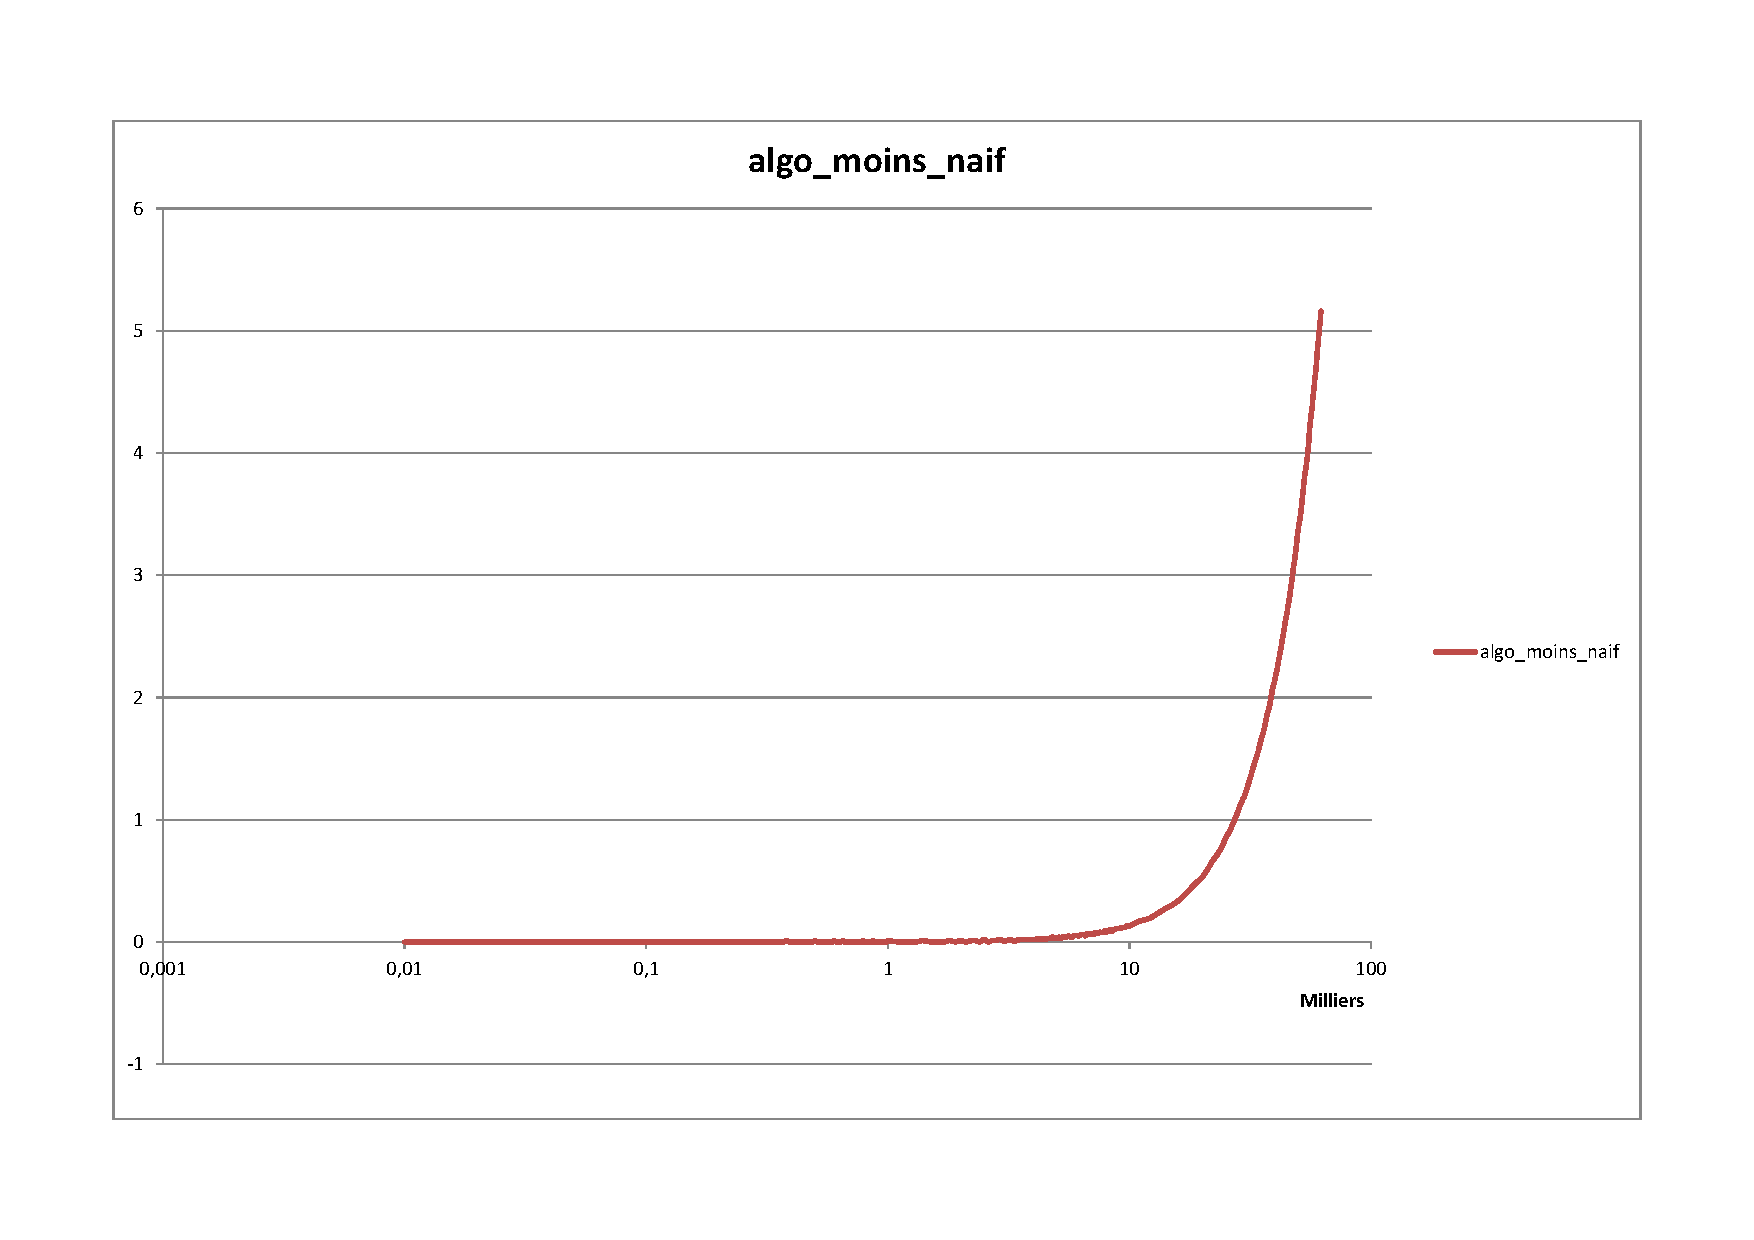
\includegraphics [scale=0.5]{images/algo_moins_naif.png}
\caption{Performances de l'algorithme moins naïf}
\end{figure}

\begin{figure}[h]
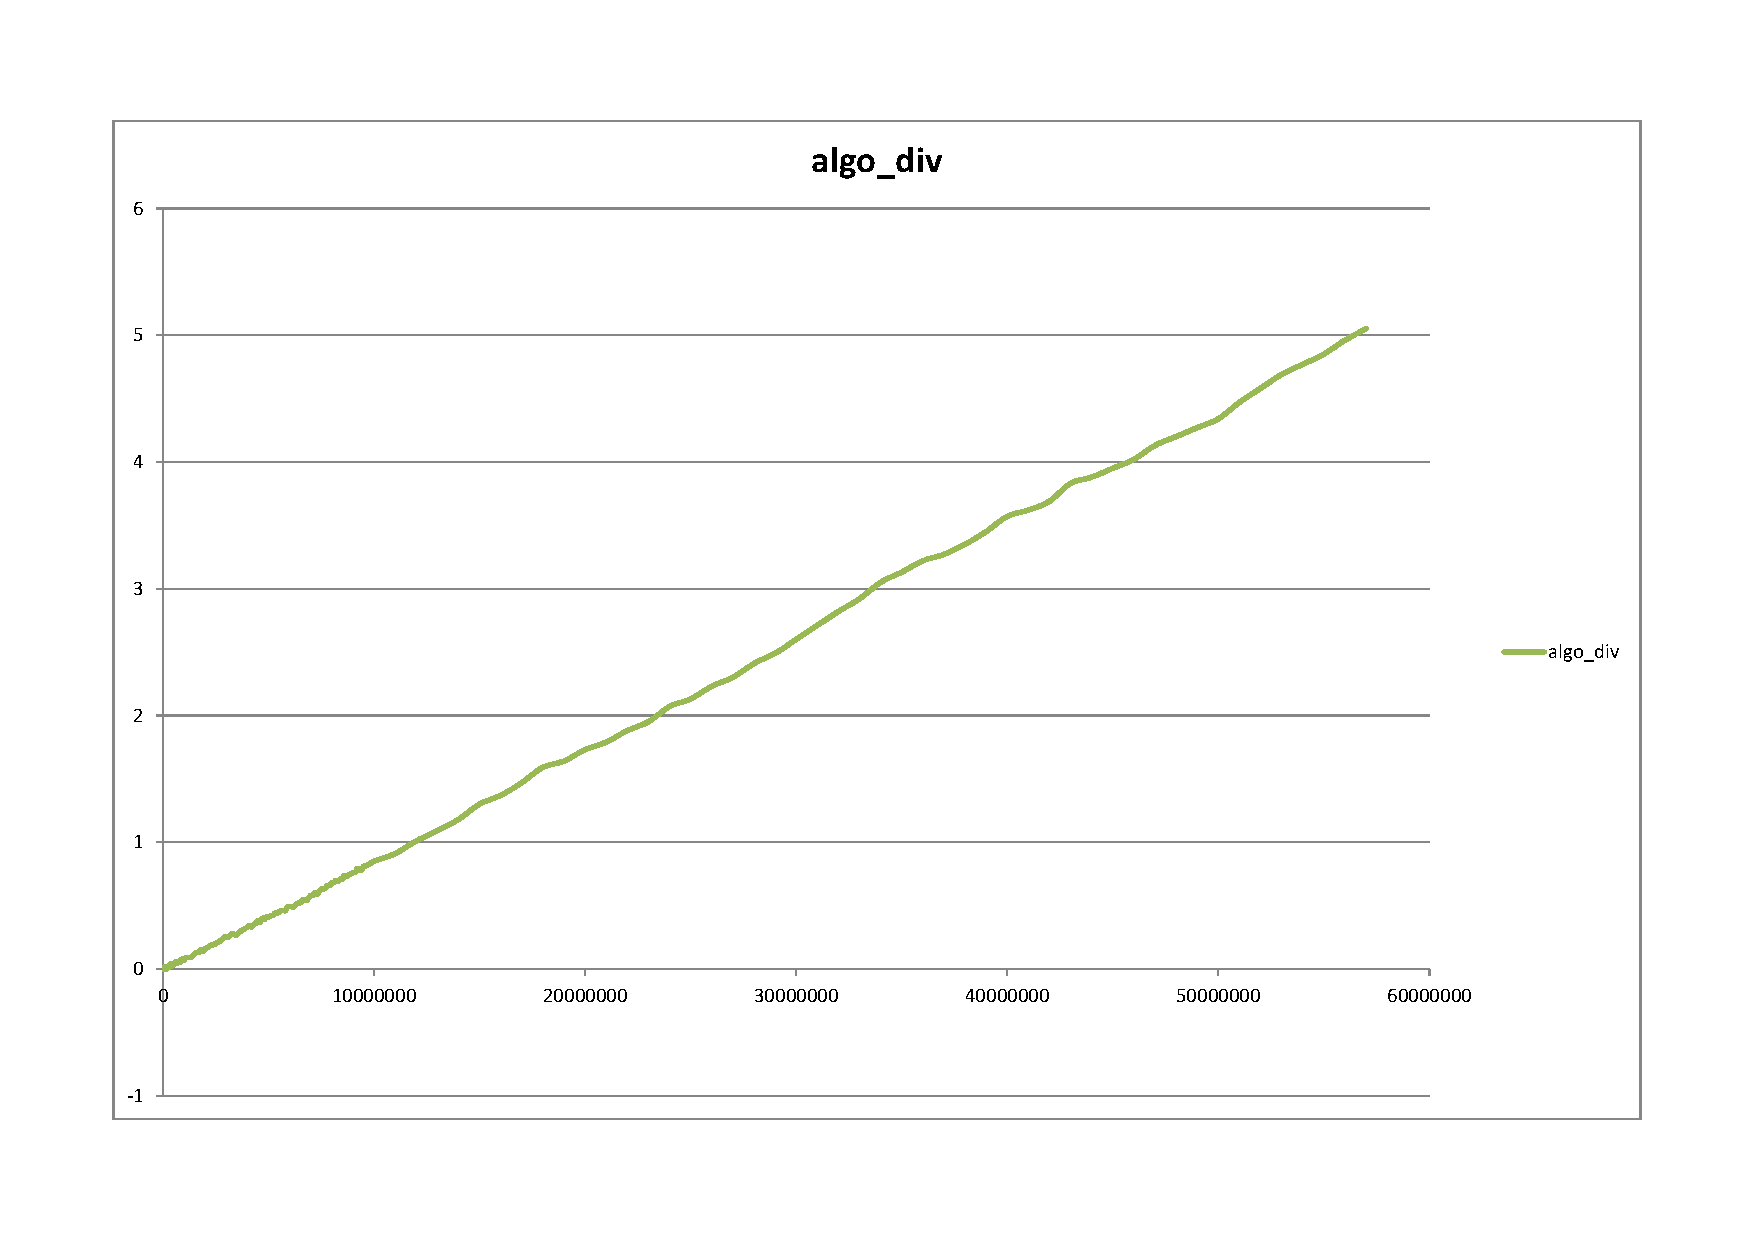
\includegraphics [scale=0.5]{images/algo_div.png}
\caption{Performances de l'algorithme diviser pour régner}
\end{figure}

\begin{figure}[h]
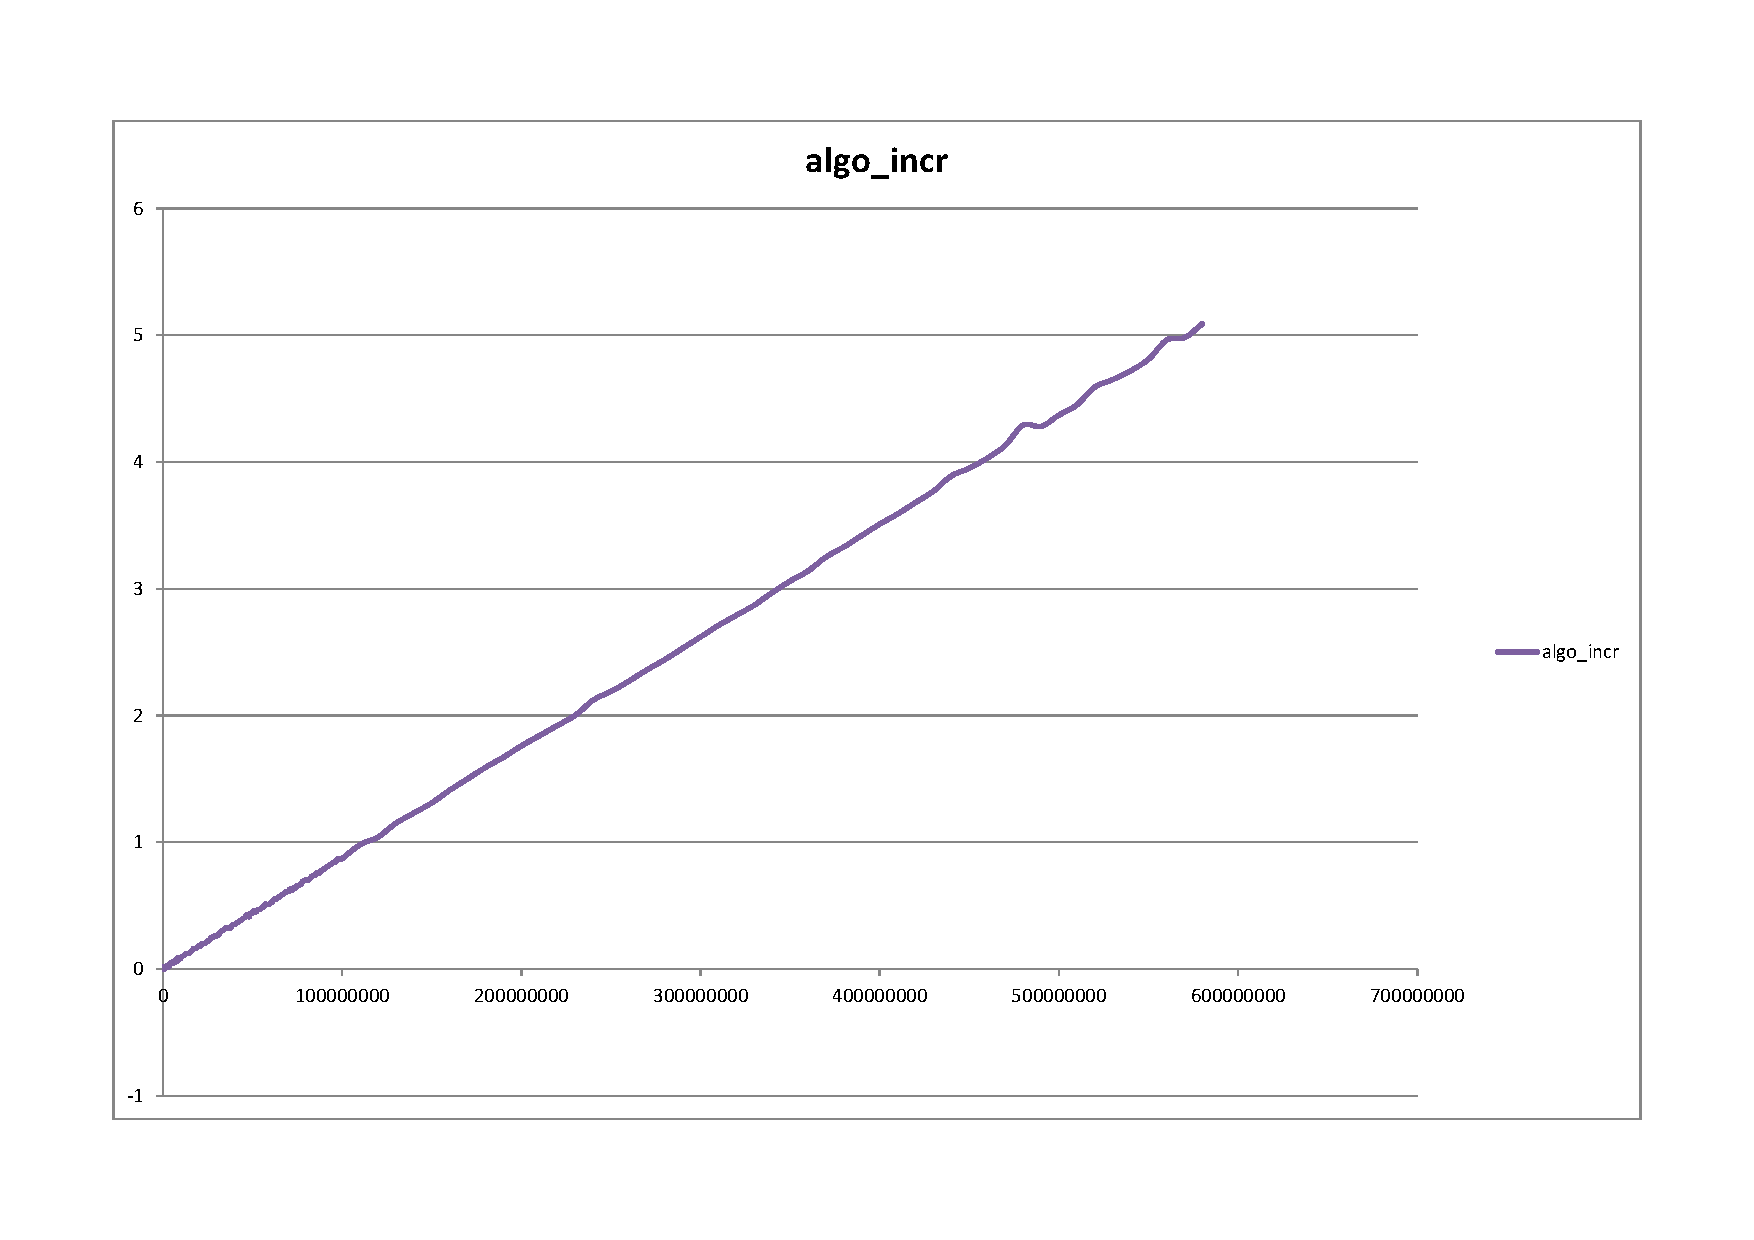
\includegraphics [scale=0.5]{images/algo_incr.png}
\caption{Performances de l'algorithme incrémental}
\end{figure}

\end{document}
